\documentclass[conference,onecolumn]{IEEEtran}
\IEEEoverridecommandlockouts
\usepackage{cite}
\usepackage{amsmath,amssymb,amsfonts}
\usepackage{algorithmic}
\usepackage{graphicx}
\usepackage{listings}
\usepackage{float}
\usepackage{textcomp}
\usepackage{gensymb}
\usepackage{xcolor}
\usepackage[spanish]{babel}

% --- Estilo de listados de codigo (borde verde, fondo blanco) ---
\definecolor{listinggreen}{RGB}{0,130,0}
\lstdefinestyle{tallerstyle}{backgroundcolor=\color{white},basicstyle=\ttfamily\footnotesize,breaklines=true,frame=single,rulecolor=\color{listinggreen},frameround=ffff,framesep=4pt,xleftmargin=6pt,xrightmargin=6pt,commentstyle=\color{gray},keywordstyle=\color{blue!70!black},stringstyle=\color{red!60!black},showstringspaces=false,columns=flexible,keepspaces=true,numbers=left,numberstyle=\tiny\color{gray}}
\lstset{style=tallerstyle}

\begin{document}

\title{Simulador de un sistema OFDM conforme a LTE: transmisi\'on de im\'agenes, canal Pedestrian A y an\'alisis Monte Carlo}

\author{\IEEEauthorblockN{Tyrone Miguel Novillo Bravo}
\IEEEauthorblockA{Facultad de Ingenier\'ia\\
Departamento de Telecomunicaciones\\
Universidad de Cuenca\\
tyrone.novillo@ucuenca.edu.ec}
\and
\IEEEauthorblockN{Freddy Eduardo L\'opez Padilla}
\IEEEauthorblockA{Facultad de Ingenier\'ia\\
Departamento de Telecomunicaciones\\
Universidad de Cuenca\\
freddy.lopez@ucuenca.edu.ec}}

\maketitle

\begin{abstract}
Este trabajo presenta el dise\~no e implementaci\'on de un simulador de un sistema OFDM conforme a la numerolog\'ia de la capa f\'isica de LTE, capaz de transmitir im\'agenes a trav\'es de una cadena completa de transmisor, canal y receptor. La forma de onda se construye con IFFT/FFT, inserci\'on de pilotos y prefijo c\'iclico, parametrizada por ancho de banda, espaciamiento entre subportadoras y tipo de CP. El canal de propagaci\'on reproduce el perfil potencia-retardo Pedestrian A (ITU-R M.1225) con desvanecimiento de Rayleigh y ruido AWGN, y el receptor recupera los s\'imbolos mediante ecualizaci\'on Zero-Forcing (ZF) con conocimiento perfecto del canal. El simulador soporta tres esquemas de modulaci\'on con codificaci\'on Gray y energ\'ia media unitaria: QPSK, 16-QAM y 64-QAM. El desempe\~no se eval\'ua estad\'isticamente mediante un an\'alisis de Monte Carlo que estima las curvas BER frente a SNR con intervalos de confianza al $95\%$ basados en la distribuci\'on $t$ de Student, y se caracteriza la relaci\'on de potencia pico a promedio (PAPR) a trav\'es de su funci\'on de distribuci\'on acumulada complementaria (CCDF). Toda la l\'ogica de procesamiento se implementa en Python y se expone a trav\'es de una interfaz web que permite configurar los par\'ametros y visualizar los resultados de forma interactiva.
\end{abstract}

\begin{IEEEkeywords}
OFDM, LTE, BER, Monte Carlo, Pedestrian A, QAM, PAPR.
\end{IEEEkeywords}

\section*{Objetivos}

\textbf{Objetivo general:} Implementar y evaluar un simulador de un sistema de comunicaciones OFDM conforme a la numerolog\'ia de LTE, que permita la transmisi\'on de im\'agenes sobre un canal Pedestrian A con desvanecimiento de Rayleigh y ruido AWGN, y caracterizar su desempe\~no mediante an\'alisis estad\'istico.

\textbf{Objetivos espec\'ificos:}
\begin{itemize}
    \item Construir la cadena completa de transmisi\'on y recepci\'on OFDM (mapeo de bits, inserci\'on de pilotos, IFFT/FFT, prefijo c\'iclico y ecualizaci\'on Zero-Forcing) parametrizada seg\'un la numerolog\'ia de LTE.
    \item Implementar los esquemas de modulaci\'on QPSK, 16-QAM y 64-QAM con codificaci\'on Gray y normalizaci\'on de energ\'ia media unitaria, y verificar su comportamiento frente a un canal selectivo en frecuencia.
    \item Estimar mediante simulaci\'on de Monte Carlo las curvas BER frente a SNR de los tres esquemas, incorporando intervalos de confianza al $95\%$ con la distribuci\'on $t$ de Student.
    \item Caracterizar la relaci\'on de potencia pico a promedio (PAPR) de la se\~nal OFDM mediante su CCDF y analizar su dependencia con los par\'ametros del sistema.
\end{itemize}

\section{Introducci\'on}

La multiplexaci\'on por divisi\'on de frecuencias ortogonales (OFDM) es la t\'ecnica de transmisi\'on multiportadora del enlace descendente de LTE y un pilar de las comunicaciones m\'oviles de banda ancha. Al dividir un canal de banda ancha en numerosas subportadoras de banda estrecha transmitidas en paralelo, convierte un canal selectivo en frecuencia en un conjunto de subcanales aproximadamente planos, lo que simplifica la ecualizaci\'on y aporta robustez frente al multitrayecto; su implementaci\'on eficiente mediante la transformada r\'apida de Fourier explica su adopci\'on en LTE y las generaciones posteriores.

En este trabajo se desarroll\'o un simulador OFDM conforme a la numerolog\'ia de LTE que reproduce la cadena completa de transmisi\'on, canal y recepci\'on: carga una imagen, la convierte en bits, la modula con QPSK, 16-QAM o 64-QAM, la transmite por un canal Pedestrian A con desvanecimiento de Rayleigh y ruido AWGN, y la recupera mediante ecualizaci\'on Zero-Forcing, todo desde una interfaz web interactiva. La evaluaci\'on cuantifica el efecto del orden de modulaci\'on y de la SNR sobre la calidad de la imagen recuperada y la tasa de error de bit (BER), estima las curvas BER frente a SNR mediante un an\'alisis de Monte Carlo con intervalos de confianza al $95\%$ basados en la distribuci\'on $t$ de Student, y caracteriza la relaci\'on de potencia pico a promedio (PAPR) mediante su CCDF.

\section{Marco te\'orico}

\subsection{Modulaci\'on OFDM, IFFT/FFT y prefijo c\'iclico}

OFDM divide un canal de banda ancha en $N$ subportadoras ortogonales de banda estrecha transmitidas en paralelo, cada una con un s\'imbolo de modulaci\'on digital a una tasa $N$ veces menor \cite{3gpp36211,cho2010mimo}. La condici\'on de ortogonalidad ($\Delta f = 1/T_u$) permite solapar sus espectros sin interferencia entre portadoras (ICI). Al estrechar cada subportadora por debajo del ancho de banda de coherencia, el canal selectivo en frecuencia se descompone en subcanales aproximadamente planos, cada uno ecualizable con un \'unico coeficiente $H[k]$ \cite{goldsmith2005wireless}. La generaci\'on y demodulaci\'on se realizan eficientemente con la IFFT/FFT:
\begin{equation}
x[n] = \frac{1}{\sqrt{N_{FFT}}}\sum_{k=0}^{N_{FFT}-1} X[k]\, e^{\,j 2\pi k n / N_{FFT}}.
\end{equation}
El tama\~no de la transformada $N_{FFT}$ es la menor potencia de dos $\ge N_{SC}$ (subportadoras \'utiles); la componente DC se deja nula y las posiciones restantes act\'uan como banda de guarda. La frecuencia de muestreo es $f_s = N_{FFT}\,\Delta f$.

A cada s\'imbolo se le antepone un prefijo c\'iclico (CP), copia de sus \'ultimas $N_{CP}$ muestras, que absorbe la dispersi\'on por retardo, evita la interferencia entre s\'imbolos (ISI) y convierte la convoluci\'on del canal en circular, garantizando $Y[k]=H[k]X[k]$. El s\'imbolo dura $T_{sym}=(N_{FFT}+N_{CP})/f_s$, con $N_{CP}=\mathrm{round}(T_{CP}\,f_s)$. La numerolog\'ia de LTE \cite{3gpp36211} fija $\Delta f = 15$~kHz (y $7{,}5$~kHz para difusi\'on), anchos de banda de $1{,}4$ a $20$~MHz mapeados a $N_{SC}$ entre $72$ y $1200$ (hasta $2400$ con $7{,}5$~kHz), CP normal ($4{,}7~\mu$s) o extendido ($16{,}67$/$33{,}33~\mu$s), y subportadoras piloto con densidad de una de cada doce.

\subsection{Modulaciones digitales: QPSK, 16-QAM y 64-QAM}

Cada esquema asigna $m=\log_2 M$ bits a un punto de una constelaci\'on $I$--$Q$: QPSK ($m{=}2$), 16-QAM ($m{=}4$, dos 4-PAM) y 64-QAM ($m{=}6$, dos 8-PAM) \cite{proakis2008digital}. Se emplea codificaci\'on Gray ---s\'imbolos vecinos difieren en un solo bit, minimizando los errores de bit--- y se normaliza la energ\'ia media a la unidad dividiendo por $\sqrt{2}$, $\sqrt{10}$ y $\sqrt{42}$, respectivamente. A mayor orden $M$ se gana eficiencia espectral ($\log_2 M$ bits/s\'imbolo), pero se reduce la distancia m\'inima entre s\'imbolos ($d_{\min}$ pasa de $\sqrt{2}$ en QPSK a $\approx 0{,}31$ en 64-QAM), por lo que la BER empeora a igual SNR. La detecci\'on es por decisi\'on dura (m\'inima distancia). Este compromiso fundamenta la modulaci\'on y codificaci\'on adaptativas (AMC): se usa 64-QAM cerca de la estaci\'on base (SNR alta) y QPSK en el borde de celda (SNR baja) \cite{goldsmith2005wireless}.

\subsection{Canal Pedestrian A, ruido AWGN y ecualizaci\'on}

En propagaci\'on m\'ovil sin l\'inea de vista, la superposici\'on de m\'ultiples trayectorias produce desvanecimiento de Rayleigh y selectividad en frecuencia \cite{rappaport2002}. Se adopta el perfil potencia-retardo Pedestrian~A (ITU-R M.1225) \cite{ituR1225}, de cuatro taps (Tabla~\ref{tab:pedA}); cada tap es un coeficiente gaussiano complejo de media nula y la respuesta en frecuencia $H[k]$ se obtiene por FFT de la respuesta al impulso.

\begin{table}[H]
    \renewcommand{\arraystretch}{1.2}
    \caption{Perfil potencia-retardo del modelo Pedestrian A \cite{ituR1225}.}
    \label{tab:pedA}
    \centering
    \begin{tabular}{ccc}
        \hline
        \textbf{Tap} & \textbf{Retardo (ns)} & \textbf{Potencia (dB)} \\
        \hline
        1 & 0   & 0       \\
        2 & 110 & -9{,}7  \\
        3 & 190 & -19{,}2 \\
        4 & 410 & -22{,}8 \\
        \hline
    \end{tabular}
\end{table}

El receptor observa, en cada subportadora,
\begin{equation}
Y[k]=H[k]\,X[k]+N[k], \label{eq:rx_model}
\end{equation}
donde $N[k]\sim\mathcal{CN}(0,\sigma_N^2)$ es ruido AWGN con potencia $\sigma_N^2 = P_s/10^{\,SNR_{dB}/10}$. Disponiendo del canal, la ecualizaci\'on Zero-Forcing estima
\begin{equation}
\hat{X}[k]=\frac{Y[k]}{H[k]}=X[k]+\frac{N[k]}{H[k]}, \label{eq:zf}
\end{equation}
que elimina la distorsi\'on del canal a costa de amplificar el ruido donde $|H[k]|$ es peque\~no. Sin ecualizar, la fase aleatoria de $H[k]$ rota los s\'imbolos y la BER se satura en $\approx 0{,}5$ aunque aumente la SNR; de ah\'i que la ecualizaci\'on sea imprescindible en este canal \cite{goldsmith2005}.

\subsection{M\'etricas: BER, Monte Carlo, IC $t$ de Student y PAPR}

La tasa de error de bit, $\mathrm{BER}=N_e/N_b$ (bits err\'oneos entre transmitidos), decrece mon\'otonamente con la SNR y empeora con el orden de modulaci\'on \cite{proakis2008}. Al no existir una expresi\'on cerrada para un canal Rayleigh, la BER se estima por simulaci\'on de Monte Carlo: se promedian $n=10$ corridas independientes por punto de SNR ($0$ a $15$~dB), con $50\,000$ bits aleatorios cada una. La incertidumbre se cuantifica con un intervalo de confianza basado en la distribuci\'on $t$ de Student (muestra peque\~na y varianza desconocida):
\begin{equation}
\mathrm{IC}_{95\%}=\overline{\mathrm{BER}}\;\pm\; t_{0{,}025,\,9}\,\frac{s}{\sqrt{n}},
\end{equation}
con $n-1=9$ grados de libertad, y se representa como barras de error sobre cada punto. Por \'ultimo, la relaci\'on de potencia pico a promedio y su funci\'on de distribuci\'on acumulada complementaria,
\begin{equation}
\mathrm{PAPR}=\frac{\max_n |x[n]|^2}{\mathbb{E}[\,|x[n]|^2\,]}, \qquad \mathrm{CCDF}(\mathrm{PAPR}_0)=\Pr\{\mathrm{PAPR}>\mathrm{PAPR}_0\},
\end{equation}
caracterizan los picos de la se\~nal OFDM ---suma coherente de subportadoras v\'ia IFFT--- que obligan a un margen de retroceso (\textit{back-off}) en el amplificador de potencia. La CCDF es pr\'acticamente independiente de la modulaci\'on y depende sobre todo del n\'umero de subportadoras \cite{han2005}.

\section{Metodolog\'ia -- Desarrollo de la pr\'actica}

Toda la l\'ogica de procesamiento del simulador se implementa en un \'unico m\'odulo \texttt{app.py} escrito en Python, apoy\'andose en las bibliotecas \texttt{numpy} para el c\'alculo num\'erico vectorizado (FFT/IFFT, generaci\'on de canal y ruido), \texttt{scipy} para las herramientas estad\'isticas (valor cr\'itico de la distribuci\'on $t$ de Student) y \texttt{Pillow} para la lectura y reconstrucci\'on de las im\'agenes transmitidas. Esta l\'ogica se expone al usuario mediante una interfaz web servida con Flask, que permite configurar los par\'ametros de la cadena, lanzar las transmisiones y los an\'alisis, y visualizar los resultados de forma interactiva. A continuaci\'on se describen las funciones principales que conforman la cadena de transmisi\'on, canal y recepci\'on.

\subsection{Arquitectura general de la cadena TX$\rightarrow$Canal$\rightarrow$RX}

La funci\'on \texttt{cadena\_tx\_rx} constituye el n\'ucleo del simulador y ejecuta el flujo completo de transmisi\'on, propagaci\'on y recepci\'on para un vector de bits dado, una modulaci\'on, un conjunto de par\'ametros OFDM, un valor de SNR y un generador aleatorio. Toda esta l\'ogica se expone mediante \emph{endpoints} Flask. El procesamiento se realiza por bloques: los bits se mapean a s\'imbolos QAM/QPSK, se rellenan (\emph{padding}) hasta completar un n\'umero entero de s\'imbolos OFDM y se itera s\'imbolo a s\'imbolo aplicando sucesivamente modulaci\'on OFDM, canal selectivo en frecuencia, ruido aditivo y recepci\'on con ecualizaci\'on.

\begin{lstlisting}[language=Python]
for i in range(n_ofdm):
    bloque_datos = simbolos_qam[i*n_datos:(i+1)*n_datos]
    rejilla = insertar_pilotos(bloque_datos, n_sc)
    senal_t, indices_fft = modulacion_ofdm(rejilla, n_fft, n_cp)
    H = generar_canal_pedestrian_a(n_fft, fs, indices_fft, rng)
    rejilla_freq = rejilla * H
    senal_canal, _ = modulacion_ofdm(rejilla_freq, n_fft, n_cp)
    senal_rx = agregar_ruido_awgn(senal_canal, snr_db, rng)
    rejilla_rx = demodulacion_ofdm(senal_rx, indices_fft, n_fft, n_cp, n_sc)
    rejilla_eq = rejilla_rx / H
    datos_rx = rejilla_eq[indices_datos_sc]
    bits_rx_total.append(mod["demapear"](datos_rx))
\end{lstlisting}

El bucle integra la totalidad de la cadena: cada s\'imbolo OFDM atraviesa el bloque transmisor (\texttt{insertar\_pilotos}, \texttt{modulacion\_ofdm}), el canal Pedestrian~A aplicado en el dominio de la frecuencia, el ruido AWGN (\texttt{agregar\_ruido\_awgn}) y el bloque receptor (\texttt{demodulacion\_ofdm}) con ecualizaci\'on \emph{Zero-Forcing}. Conviene precisar que, al aplicarse el canal directamente como producto en frecuencia ($\texttt{rejilla\_freq = rejilla * H}$), el modelo equivale a un canal plano por subportadora seg\'un \eqref{eq:rx_model}; en esta implementaci\'on no se realiza una convoluci\'on temporal multitrayecto expl\'icita, por lo que el prefijo c\'iclico se a\~nade y se descarta para mantener la coherencia de la cadena pero no act\'ua de forma funcional como mitigador de ISI. Finalmente, los bits recuperados se concatenan, se recortan al tama\~no original transmitido y se calcula la tasa de error de bit (BER) mediante \texttt{calcular\_ber}.

\subsection{Mapeo de bits a s\'imbolos}

El simulador implementa tres esquemas de modulaci\'on con codificaci\'on Gray y normalizaci\'on de energ\'ia media unitaria ($E_s = 1$): QPSK, 16-QAM y 64-QAM, mediante las funciones \texttt{qpsk\_mapear}, \texttt{qam16\_mapear} y \texttt{qam64\_mapear}, respectivamente. El mapeo Gray garantiza que s\'imbolos adyacentes difieran en un solo bit, minimizando la propagaci\'on de errores. La normalizaci\'on divide cada s\'imbolo por la ra\'iz de su energ\'ia promedio ($\sqrt{2}$ para QPSK, $\sqrt{10}$ para 16-QAM y $\sqrt{42}$ para 64-QAM).

\begin{lstlisting}[language=Python]
def qpsk_mapear(bits):
    bits = bits.reshape(-1, 2).astype(np.int8)
    i = 1 - 2 * bits[:, 0]   # Gray: 0 -> +1, 1 -> -1
    q = 1 - 2 * bits[:, 1]
    return (i + 1j * q) / np.sqrt(2)

# Mapa Gray 4-PAM (16-QAM): 2 bits -> nivel {-3,-1,+1,+3}
_GRAY_4 = {(0, 0): -3, (0, 1): -1, (1, 1): 1, (1, 0): 3}
\end{lstlisting}

La funci\'on \texttt{qpsk\_mapear} agrupa los bits en pares, asignando cada bit a las componentes en fase ($I$) y cuadratura ($Q$) seg\'un la regla Gray $0\!\rightarrow\!+1$, $1\!\rightarrow\!-1$, y normaliza por $\sqrt{2}$. Para 16-QAM y 64-QAM se reutiliza el principio de modulaci\'on PAM independiente por eje: el diccionario \texttt{\_GRAY\_4} asocia cada par de bits a un nivel de la constelaci\'on 4-PAM $\{-3,-1,+1,+3\}$, mientras que \texttt{\_GRAY\_8} hace lo propio sobre 8-PAM para 64-QAM. El demapeo correspondiente (\texttt{qpsk\_demapear}, \texttt{qam16\_demapear}, \texttt{qam64\_demapear}) aplica decisi\'on dura (\emph{hard-decision}) buscando el nivel m\'as cercano.

\subsection{Construcci\'on del s\'imbolo OFDM}

La conformaci\'on de cada s\'imbolo OFDM se compone de tres etapas: inserci\'on de pilotos, mapeo de subportadoras al vector de IFFT y transformada inversa con adici\'on del prefijo c\'iclico. La funci\'on \texttt{insertar\_pilotos} ubica un piloto de valor $1+0j$ cada \texttt{PASO\_PILOTO}~$=12$ subportadoras (densidad $1/12$), colocando los s\'imbolos de datos en las posiciones restantes; los \'indices de pilotos y datos se obtienen con \texttt{indices\_pilotos\_datos}. Posteriormente, \texttt{mapeo\_sc\_a\_fft} distribuye las $N_{SC}$ subportadoras activas sobre el vector de $N_{FFT}$ puntos, dejando vac\'ia la componente DC y centrando los \'indices en $[-N_{SC}/2,\dots,-1,+1,\dots,+N_{SC}/2]$.

\begin{lstlisting}[language=Python]
def modulacion_ofdm(rejilla_sc, n_fft, n_cp):
    """IFFT + CP."""
    vec_freq, indices_fft = mapeo_sc_a_fft(rejilla_sc, n_fft)
    senal_t = np.fft.ifft(vec_freq) * n_fft / np.sqrt(len(rejilla_sc))
    cp = senal_t[-n_cp:] if n_cp > 0 else np.array([], dtype=complex)
    return np.concatenate([cp, senal_t]), indices_fft
\end{lstlisting}

La funci\'on \texttt{modulacion\_ofdm} obtiene primero el vector espectral mediante \texttt{mapeo\_sc\_a\_fft}, aplica la IFFT para pasar al dominio temporal con una normalizaci\'on por $N_{FFT}/\sqrt{N_{SC}}$ que preserva la energ\'ia, y antepone el prefijo c\'iclico (CP) copiando las \'ultimas \texttt{n\_cp} muestras al inicio del s\'imbolo. El CP mitiga la interferencia entre s\'imbolos provocada por la dispersi\'on temporal del canal y convierte la convoluci\'on lineal en circular, permitiendo la ecualizaci\'on por subportadora en el receptor.

\subsection{Canal Pedestrian A y ruido AWGN}

El canal multitrayecto se modela seg\'un el perfil Pedestrian~A (ITU-R M.1225), caracterizado por cuatro taps con retardos $\{0,\,110,\,190,\,410\}$~ns y potencias relativas $\{0,\,-9.7,\,-19.2,\,-22.8\}$~dB. La funci\'on \texttt{generar\_canal\_pedestrian\_a} genera coeficientes complejos gaussianos por tap (desvanecimiento Rayleigh), sit\'ua cada tap en la rejilla temporal muestreada a $f_s$ y obtiene la respuesta en frecuencia $H[k]$ mediante FFT de la respuesta impulsiva.

\begin{lstlisting}[language=Python]
def generar_canal_pedestrian_a(n_fft, fs, indices_fft, rng):
    pot_lin = 10 ** (POTENCIAS_PEDA_DB / 10)
    pot_lin = pot_lin / np.sum(pot_lin)        # potencia total = 1
    a = (rng.standard_normal(len(pot_lin)) +
         1j * rng.standard_normal(len(pot_lin))) * np.sqrt(pot_lin / 2)
    retardos_muestras = np.round(RETARDOS_PEDA_NS * 1e-9 * fs).astype(int)
    h = np.zeros(n_fft, dtype=complex)
    for tap, m in enumerate(retardos_muestras):
        if m < n_fft:
            h[m] += a[tap]
    H = np.fft.fft(h)
    return H[indices_fft]
\end{lstlisting}

Las potencias en dB se convierten a escala lineal y se normalizan para que la potencia total del canal sea unitaria; los coeficientes Rayleigh se escalan por $\sqrt{P/2}$ por componente. Los retardos se cuantizan a muestras seg\'un $f_s$ y se ensamblan en la respuesta impulsiva discreta $h$, cuya FFT proporciona $H[k]$ sobre las subportadoras activas. Por su parte, la funci\'on \texttt{agregar\_ruido\_awgn} a\~nade ruido blanco gaussiano complejo calibrado a partir del SNR especificado.

\begin{lstlisting}[language=Python]
def agregar_ruido_awgn(senal, snr_db, rng):
    pot_senal = np.mean(np.abs(senal) ** 2)
    pot_ruido = pot_senal / (10 ** (snr_db / 10))
    ruido = np.sqrt(pot_ruido / 2) * (rng.standard_normal(senal.shape) +
                                      1j * rng.standard_normal(senal.shape))
    return senal + ruido
\end{lstlisting}

\texttt{agregar\_ruido\_awgn} estima la potencia de la se\~nal, deriva la potencia de ruido requerida para el SNR objetivo mediante $P_n = P_s/10^{\,SNR/10}$ y genera ruido complejo con varianza $P_n/2$ por componente (real e imaginaria), garantizando el nivel de relaci\'on se\~nal a ruido configurado.

\subsection{Recepci\'on y ecualizaci\'on Zero-Forcing}

El bloque receptor invierte las operaciones del transmisor mediante \texttt{demodulacion\_ofdm}, que descarta el prefijo c\'iclico, aplica la FFT al s\'imbolo y extrae las $N_{SC}$ subportadoras activas con la normalizaci\'on inversa correspondiente. A continuaci\'on, dado que el canal $H[k]$ es conocido en este escenario, se aplica ecualizaci\'on \emph{Zero-Forcing} (ZF) dividiendo punto a punto la rejilla recibida por la respuesta en frecuencia del canal.

\begin{lstlisting}[language=Python]
def demodulacion_ofdm(simbolo_con_cp, indices_fft, n_fft, n_cp, n_sc):
    sin_cp = simbolo_con_cp[n_cp:n_cp + n_fft]
    espectro = np.fft.fft(sin_cp) / n_fft * np.sqrt(n_sc)
    return espectro[indices_fft]

# Dentro de cadena_tx_rx:
rejilla_rx = demodulacion_ofdm(senal_rx, indices_fft, n_fft, n_cp, n_sc)
rejilla_eq = rejilla_rx / H          # ecualizacion Zero-Forcing
datos_rx = rejilla_eq[indices_datos_sc]
\end{lstlisting}

La operaci\'on \texttt{rejilla\_eq = rejilla\_rx / H} invierte exactamente el efecto de $H[k]$, a costa de amplificar el ruido en subportadoras con desvanecimiento profundo. El receptor no estima el canal a partir de los pilotos, sino que reutiliza la respuesta $H[k]$ del transmisor (ecualizaci\'on ideal con canal conocido). Finalmente se seleccionan las posiciones de datos y los s\'imbolos ecualizados pasan al demapeador \emph{hard-decision}.

\subsection{Par\'ametros derivados de la configuraci\'on}

La funci\'on \texttt{calcular\_parametros\_ofdm} traduce la configuraci\'on de usuario (ancho de banda, espaciado entre subportadoras $\Delta f$ y tipo de CP) en los par\'ametros f\'isicos de la cadena. El n\'umero de subportadoras $N_{SC}$ se obtiene de la tabla LTE \texttt{TABLA\_NSC} indexada por la pareja $(BW,\Delta f)$; el tama\~no de la FFT se fija como la siguiente potencia de dos mayor o igual a $N_{SC}$ (\texttt{siguiente\_pot\_2}); la frecuencia de muestreo es $f_s = N_{FFT}\cdot\Delta f$; y la longitud del CP se deriva de la duraci\'on normalizada LTE (\texttt{duracion\_cp\_us}) como $N_{CP}=\mathrm{round}(\tau_{CP}\cdot f_s)$. Adicionalmente se calcula el n\'umero de pilotos ($N_{SC}/12$), de subportadoras de datos y la cantidad de s\'imbolos OFDM necesarios para transportar la carga \'util.

\subsection{Simulaci\'on Monte Carlo e intervalos de confianza t-Student}

La validaci\'on estad\'istica del desempe\~no se realiza en el \emph{endpoint} \texttt{montecarlo}, que barre las tres modulaciones (QPSK, 16-QAM, 64-QAM) sobre $16$ valores de SNR ($0$ a $15$~dB) ejecutando $n_{sim}=10$ corridas independientes con bits aleatorios por cada combinaci\'on. Para cada punto se promedia la BER y se construye un intervalo de confianza al $95\%$ empleando la distribuci\'on t-Student con $n_{sim}-1=9$ grados de libertad, cuyo valor cr\'itico se obtiene con \texttt{scipy.stats.t.ppf(0.975, df=9)}.

\begin{lstlisting}[language=Python]
t_critico = float(t_student.ppf(0.975, df=n_sim - 1))
...
bers = np.array(bers)
mu = float(np.mean(bers))
sd = float(np.std(bers, ddof=1)) if n_sim > 1 else 0.0
margen = t_critico * sd / np.sqrt(n_sim)
ber_prom.append(mu)
ic_inf.append(max(mu - margen, 1e-6))
ic_sup.append(mu + margen)
\end{lstlisting}

El margen del intervalo es $t_{0.975,9}\cdot s/\sqrt{n_{sim}}$, con $s$ la desviaci\'on est\'andar muestral (\texttt{ddof=1}); el l\'imite inferior se acota a $10^{-6}$ para su representaci\'on en escala logar\'itmica.

\subsection{An\'alisis de PAPR mediante CCDF}

La relaci\'on entre potencia de pico y potencia media (PAPR) es una m\'etrica cr\'itica en OFDM por su impacto en la linealidad del amplificador. La funci\'on \texttt{calcular\_papr\_simbolo} eval\'ua el PAPR en decibelios de un s\'imbolo OFDM en el dominio temporal (sin CP), y \texttt{calcular\_papr\_ccdf} estima la funci\'on de distribuci\'on complementaria (CCDF) generando $1500$ s\'imbolos OFDM aleatorios por modulaci\'on, de modo que $\mathrm{CCDF}(x)=\Pr\{\mathrm{PAPR}>x\}$.

\begin{lstlisting}[language=Python]
def calcular_papr_simbolo(senal_tiempo):
    pot_pico = np.max(np.abs(senal_tiempo) ** 2)
    pot_media = np.mean(np.abs(senal_tiempo) ** 2)
    if pot_media <= 0:
        return 0.0
    return float(10 * np.log10(pot_pico / pot_media))
\end{lstlisting}

\texttt{calcular\_papr\_simbolo} calcula la potencia instant\'anea m\'axima y la potencia media del s\'imbolo y devuelve su cociente en dB mediante $10\log_{10}(P_{pico}/P_{media})$. La CCDF resultante caracteriza la probabilidad de exceder un nivel de PAPR determinado, permitiendo comparar las distintas modulaciones; al depender principalmente del n\'umero de subportadoras y no de la SNR, este an\'alisis se calcula de forma independiente al barrido de ruido.

\section{Evaluaci\'on -- An\'alisis de resultados}

En esta secci\'on se analizan los resultados obtenidos con el simulador OFDM. En primer lugar se describe la interfaz web y el panel de configuraci\'on de par\'ametros del sistema; a continuaci\'on se examinan varias transmisiones de una misma imagen empleando distintas modulaciones (64-QAM, 16-QAM y QPSK) y valores de SNR, observando el efecto del orden de modulaci\'on y del ruido sobre la calidad de la imagen recuperada y sobre la BER. Posteriormente se inspeccionan la constelaci\'on recibida tras la ecualizaci\'on Zero-Forcing y el mapa de subportadoras (respuesta en frecuencia del canal Pedestrian~A). Finalmente se discuten las curvas BER frente a SNR obtenidas mediante el an\'alisis de Monte Carlo, con sus intervalos de confianza al $95\%$ basados en la distribuci\'on $t$ de Student, y la CCDF de la PAPR para los tres esquemas de modulaci\'on.

\subsection{Interfaz del simulador y par\'ametros de configuraci\'on}

La Fig.~\ref{fig:interfaz} presenta la interfaz web del simulador. El panel lateral izquierdo permite seleccionar el ancho de banda ($5$~MHz), el espaciamiento entre subportadoras ($\Delta f = 15$~kHz) y el tipo de prefijo c\'iclico (normal), as\'i como la SNR del enlace. El \'area central incluye un mapa de cobertura con tres anillos conc\'entricos que asocian la modulaci\'on a la distancia respecto a la estaci\'on base: 64-QAM en la zona interior ($0$--$300$~m), 16-QAM en la zona intermedia ($300$--$800$~m) y QPSK en el borde de celda ($800$--$1500$~m). Al desplazar el punto que representa al equipo de usuario, el simulador selecciona autom\'aticamente la modulaci\'on correspondiente, reproduciendo el principio de modulaci\'on y codificaci\'on adaptativas de LTE.

\begin{figure}[H]
\centering
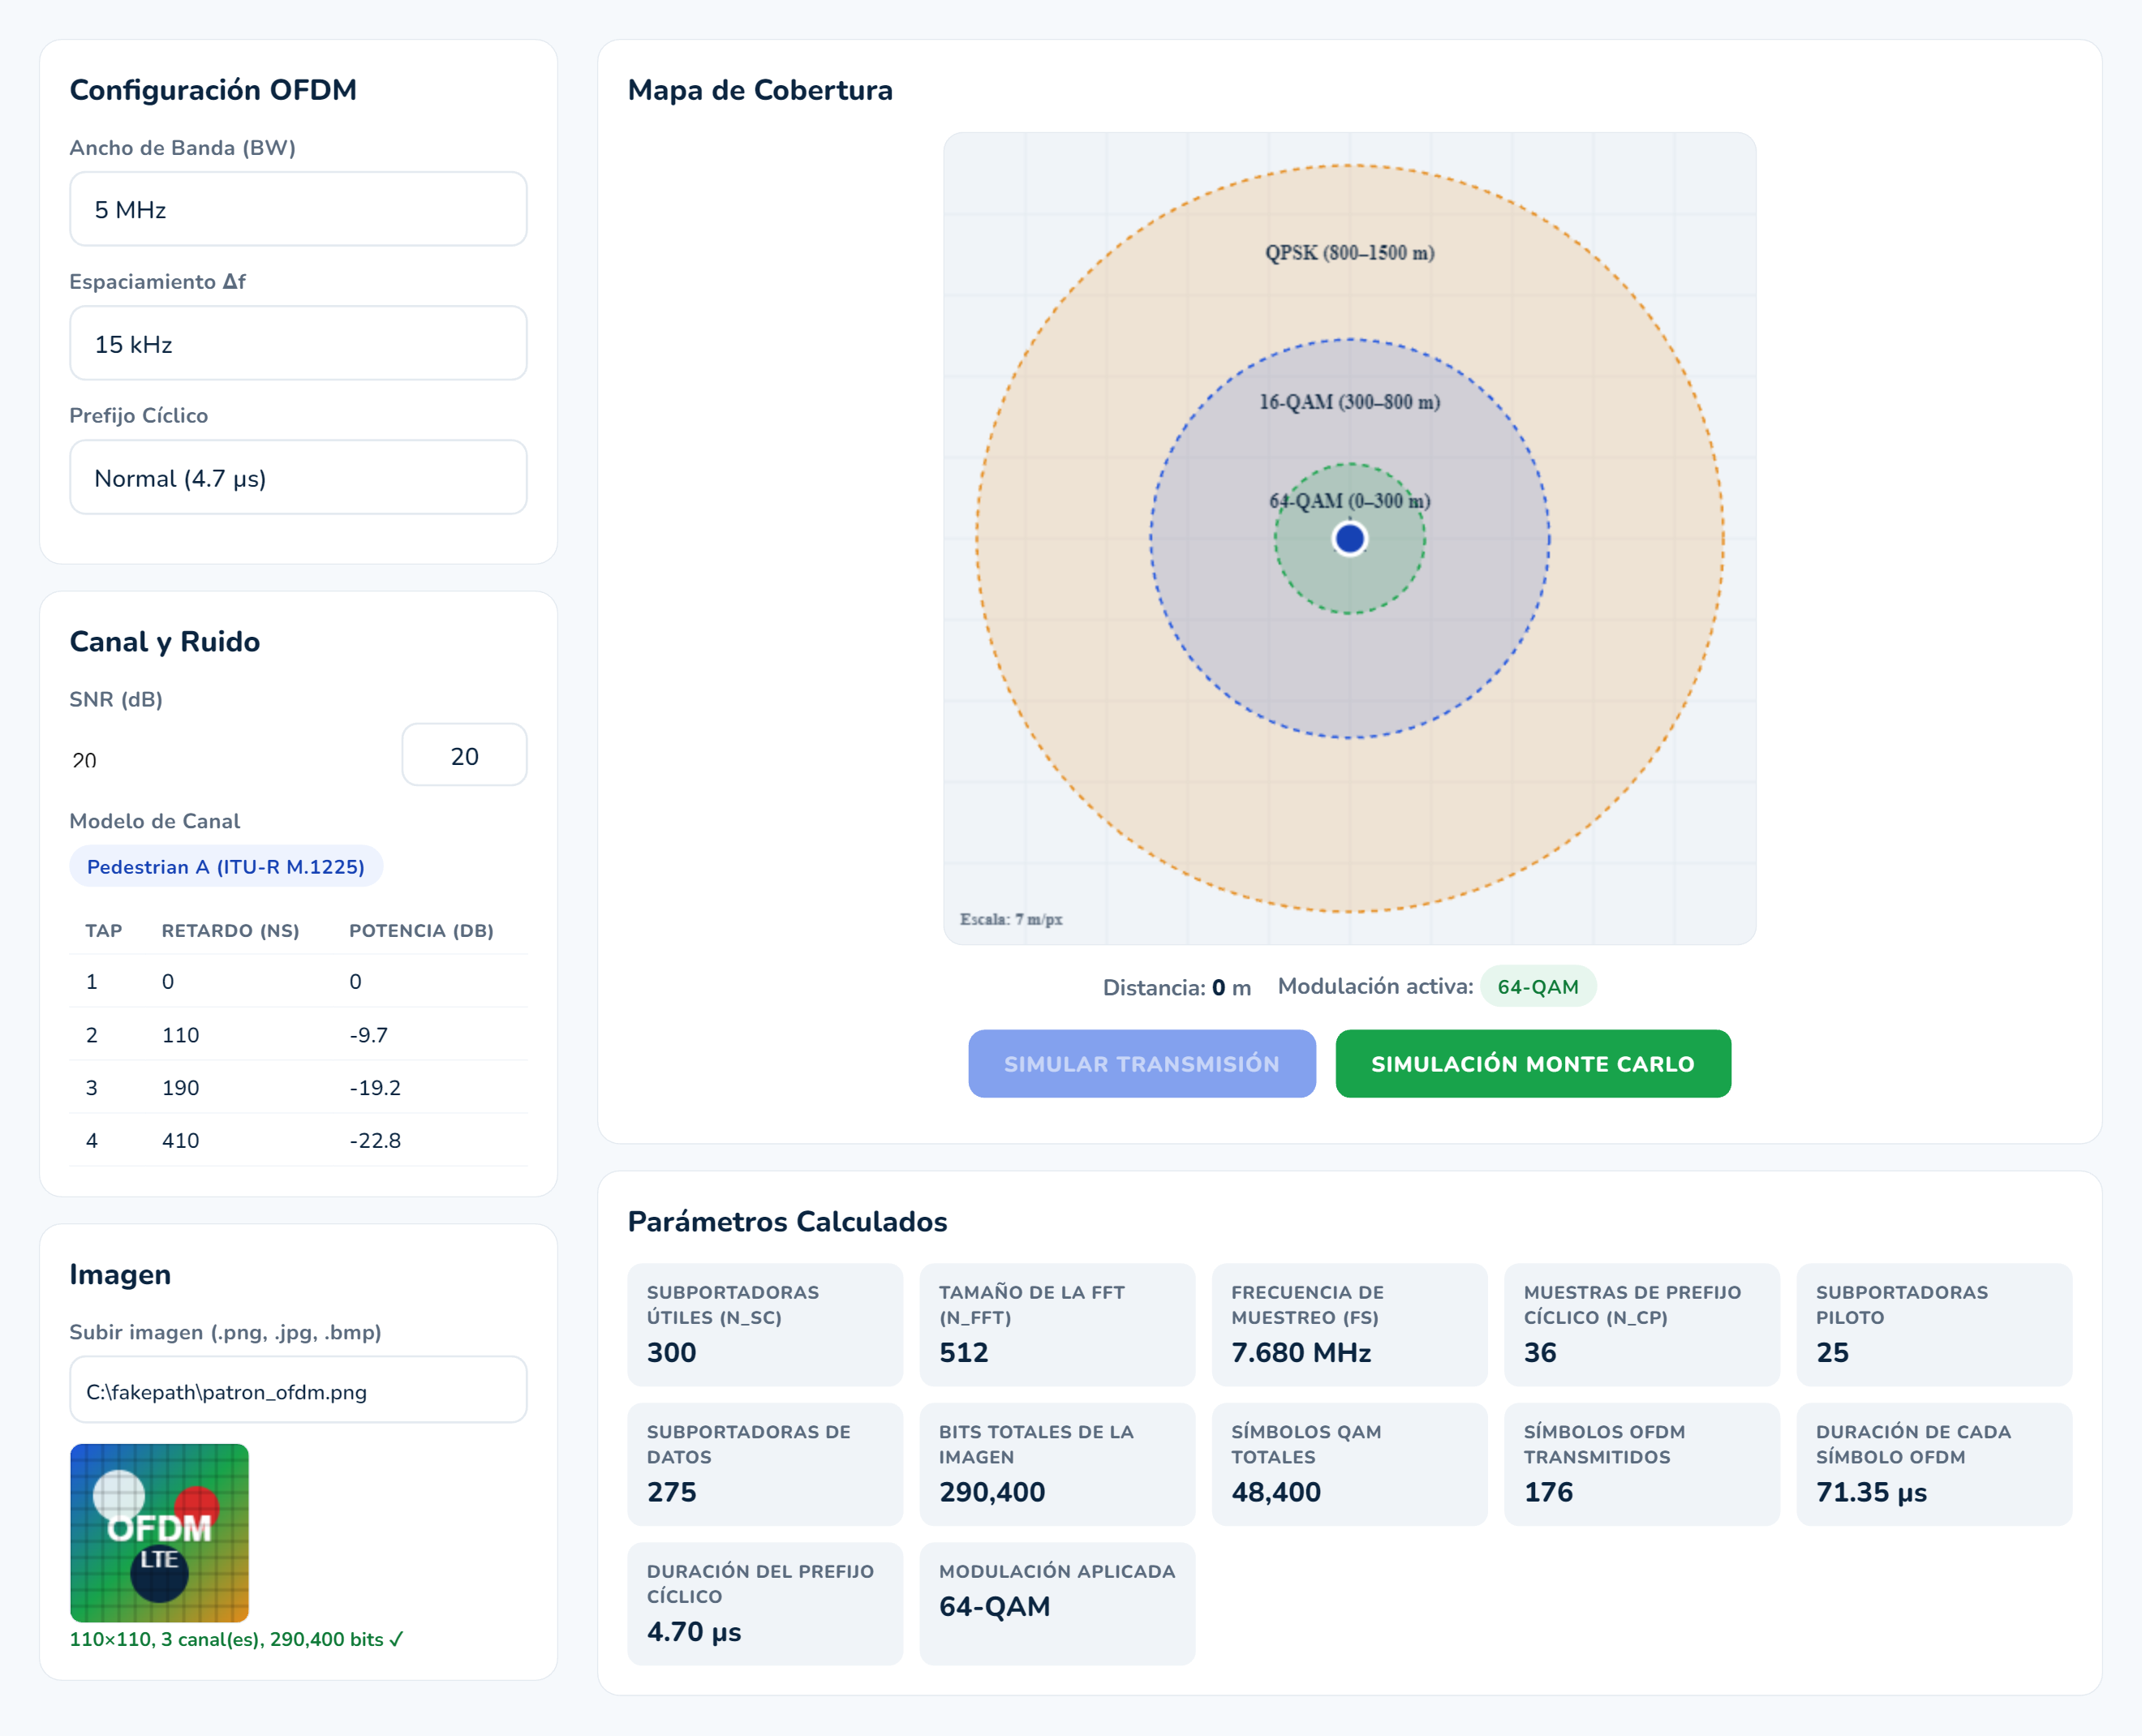
\includegraphics[width=0.95\textwidth]{img/interfaz.png}
\caption{Interfaz general del simulador OFDM-LTE: panel de configuraci\'on, mapa de cobertura con las zonas de modulaci\'on y botones de simulaci\'on.}
\label{fig:interfaz}
\end{figure}

Para la imagen de prueba empleada ($110\times110$ p\'ixeles, $3$ canales, equivalente a $290\,400$ bits), la Fig.~\ref{fig:params} resume los par\'ametros derivados de la configuraci\'on. El n\'umero de subportadoras \'utiles es $N_{SC}=300$, valor que conduce a un tama\~no de FFT $N_{FFT}=512$ (la menor potencia de dos mayor o igual que $N_{SC}$) y a una frecuencia de muestreo $f_s = N_{FFT}\cdot\Delta f = 7{,}680$~MHz. La duraci\'on del prefijo c\'iclico normal de $4{,}7~\mu$s equivale a $N_{CP}=36$ muestras. De las $300$ subportadoras, $25$ se reservan como piloto (una de cada doce) y $275$ transportan datos.

\begin{figure}[H]
\centering
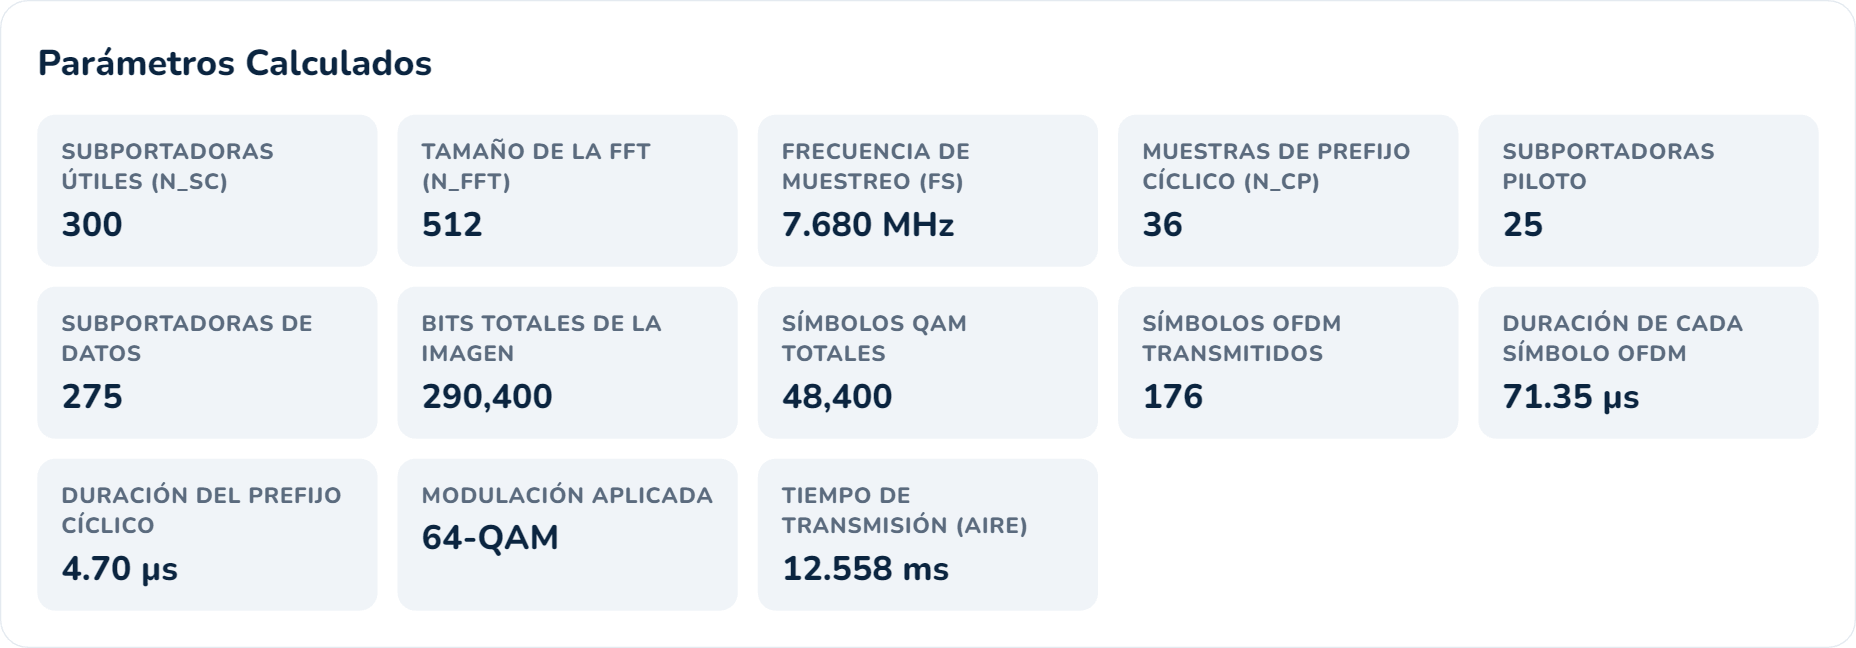
\includegraphics[width=0.95\textwidth]{img/params_calculados.png}
\caption{Panel de par\'ametros calculados para $BW{=}5$~MHz, $\Delta f{=}15$~kHz y CP normal, con la imagen de $290\,400$ bits cargada.}
\label{fig:params}
\end{figure}

\subsection{Transmisi\'on de im\'agenes con distintas modulaciones}

Se transmiti\'o la misma imagen bajo tres condiciones representativas de las zonas de cobertura, resumidas en la Tabla~\ref{tab:sims}. La Fig.~\ref{fig:sim64} corresponde a 64-QAM con una SNR de $30$~dB (equipo de usuario cercano a la estaci\'on base): la imagen recuperada es pr\'acticamente id\'entica a la original, con una BER de apenas $9{,}8\times10^{-4}$ ($286$ bits err\'oneos de $290\,400$). La Fig.~\ref{fig:sim16}, con 16-QAM y SNR de $15$~dB, presenta una degradaci\'on leve en forma de ruido granular disperso, manteni\'endose la imagen totalmente reconocible (BER $8{,}5\times10^{-3}$). La Fig.~\ref{fig:simqpsk}, con QPSK y SNR de $6$~dB (borde de celda), muestra un moteado m\'as visible, aunque la imagen contin\'ua siendo legible (BER $1{,}8\times10^{-2}$), lo que evidencia la robustez de QPSK frente a condiciones adversas.

\begin{table}[H]
\centering
\caption{Resultados de las transmisiones de imagen.}
\label{tab:sims}
\begin{tabular}{|l|c|c|c|c|c|}
\hline
\textbf{Modulaci\'on} & \textbf{SNR} & \textbf{Dist.} & \textbf{BER} & \textbf{S\'imb. OFDM} & \textbf{T. aire} \\
\hline
64-QAM & $30$~dB & $0$~m & $9{,}8\times10^{-4}$ & $176$ & $12{,}56$~ms \\
16-QAM & $15$~dB & $546$~m & $8{,}5\times10^{-3}$ & $264$ & $18{,}84$~ms \\
QPSK & $6$~dB & $1099$~m & $1{,}8\times10^{-2}$ & $528$ & $37{,}68$~ms \\
\hline
\end{tabular}
\end{table}

Conviene precisar que la BER no aumenta de forma mon\'otona con el orden de modulaci\'on en la Tabla~\ref{tab:sims}, porque cada caso se evalu\'o a una SNR distinta, asociada a su zona de cobertura. As\'i, 64-QAM obtiene la menor BER gracias a su elevada SNR, mientras que QPSK, pese a ser la modulaci\'on m\'as robusta, opera a la SNR m\'as baja. El n\'umero de s\'imbolos OFDM crece al disminuir el orden de modulaci\'on (de $176$ a $528$), pues una menor cantidad de bits por s\'imbolo exige m\'as s\'imbolos para transportar los mismos $290\,400$ bits, lo que se refleja tambi\'en en un mayor tiempo de transmisi\'on.

\begin{figure}[H]
\centering
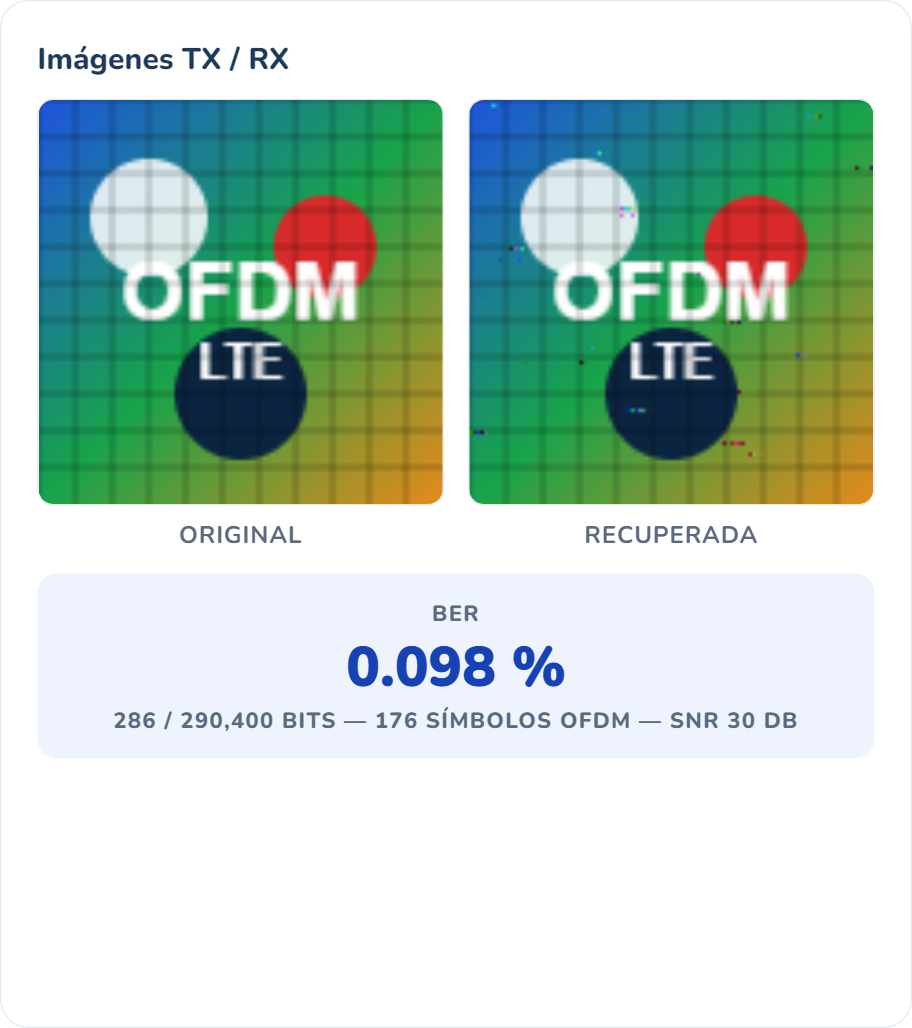
\includegraphics[width=0.8\textwidth]{img/sim_64qam.png}
\caption{Transmisi\'on con 64-QAM y SNR${=}30$~dB. La imagen recuperada es pr\'acticamente id\'entica a la original (BER ${=}9{,}8\times10^{-4}$).}
\label{fig:sim64}
\end{figure}

\begin{figure}[H]
\centering
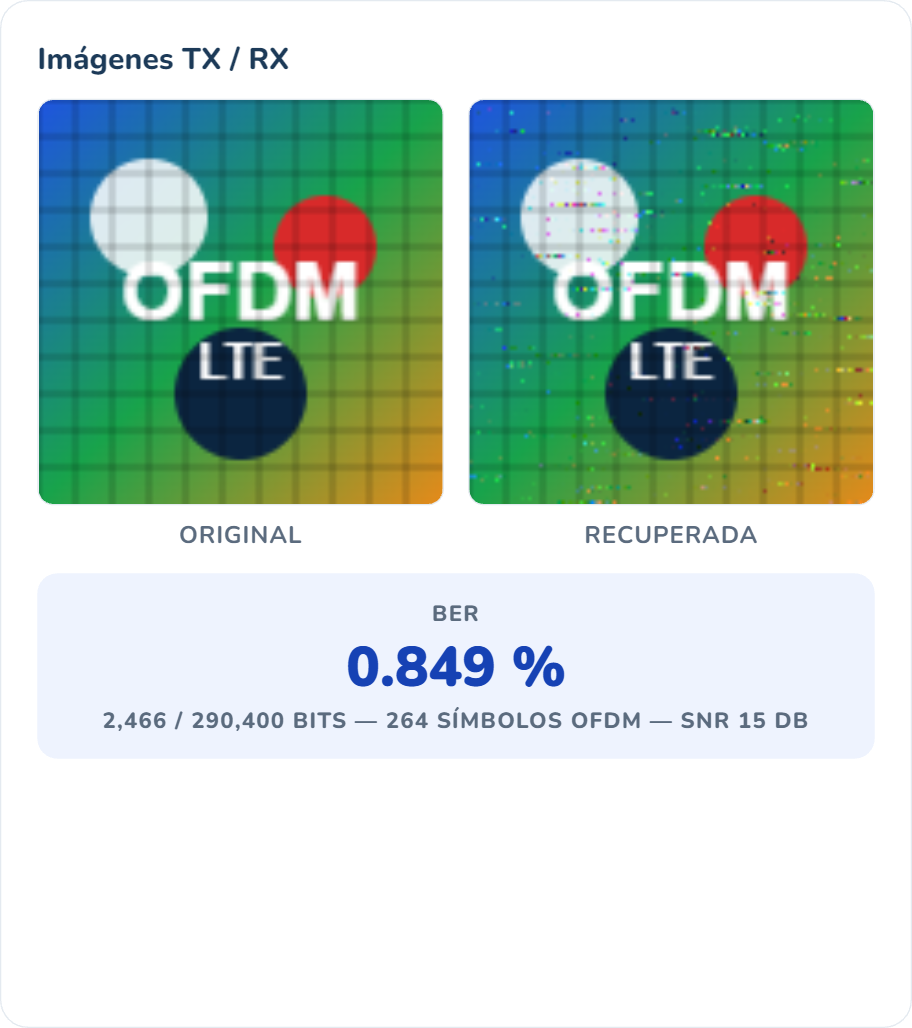
\includegraphics[width=0.8\textwidth]{img/sim_16qam.png}
\caption{Transmisi\'on con 16-QAM y SNR${=}15$~dB. Aparece ruido granular leve, pero la imagen permanece reconocible (BER ${=}8{,}5\times10^{-3}$).}
\label{fig:sim16}
\end{figure}

\begin{figure}[H]
\centering
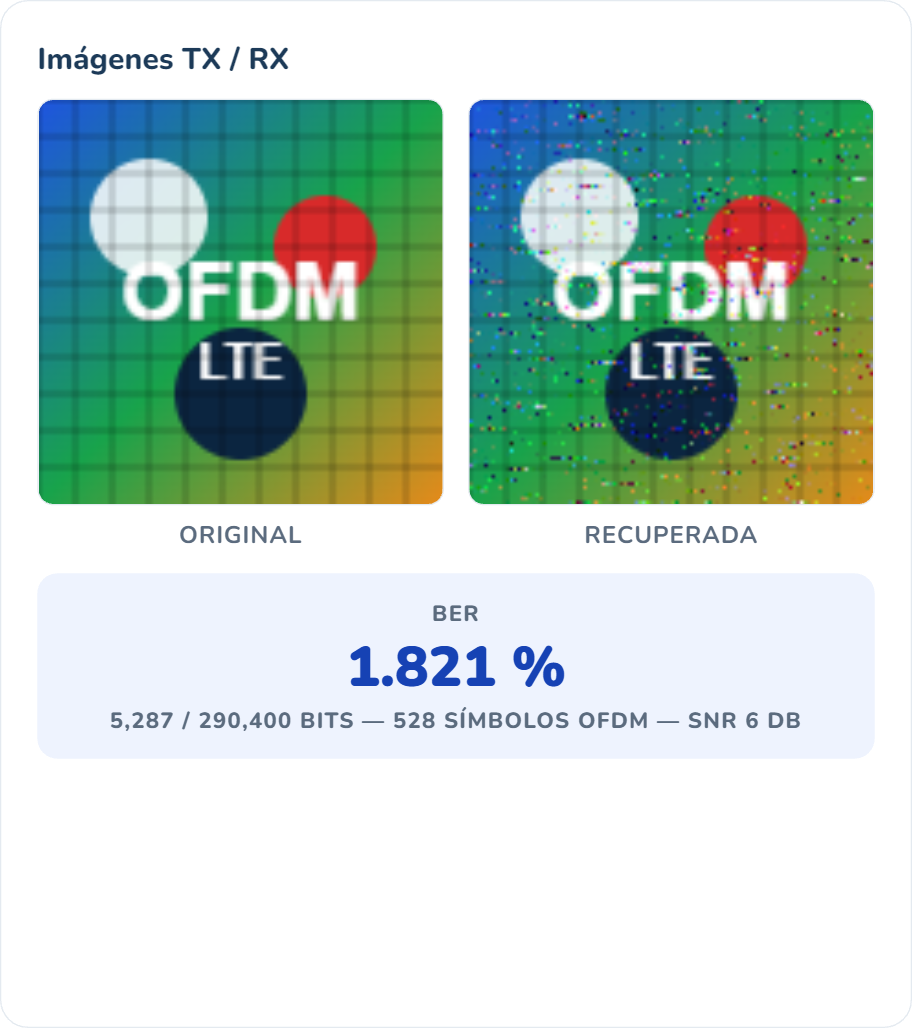
\includegraphics[width=0.8\textwidth]{img/sim_qpsk.png}
\caption{Transmisi\'on con QPSK y SNR${=}6$~dB (borde de celda). El moteado es m\'as visible, pero la imagen sigue siendo legible (BER ${=}1{,}8\times10^{-2}$).}
\label{fig:simqpsk}
\end{figure}

\subsection{Constelaci\'on recibida y mapa de subportadoras}

La Fig.~\ref{fig:const} muestra la constelaci\'on de 16-QAM recibida tras la ecualizaci\'on Zero-Forcing. Las cruces rojas indican las posiciones ideales y los puntos verdes los s\'imbolos recibidos: la ecualizaci\'on reposiciona las muestras en torno a la ret\'icula ideal, y la dispersi\'on residual alrededor de cada punto corresponde al ruido AWGN amplificado por el inverso del canal. Dicha dispersi\'on es la que origina los errores cuando un punto cruza la frontera de decisi\'on hacia un s\'imbolo vecino. La Fig.~\ref{fig:mapasc} ilustra la asignaci\'on de las $300$ subportadoras: en azul las $275$ de datos y en rojo las $25$ piloto, distribuidas una de cada doce.

\begin{figure}[H]
\centering
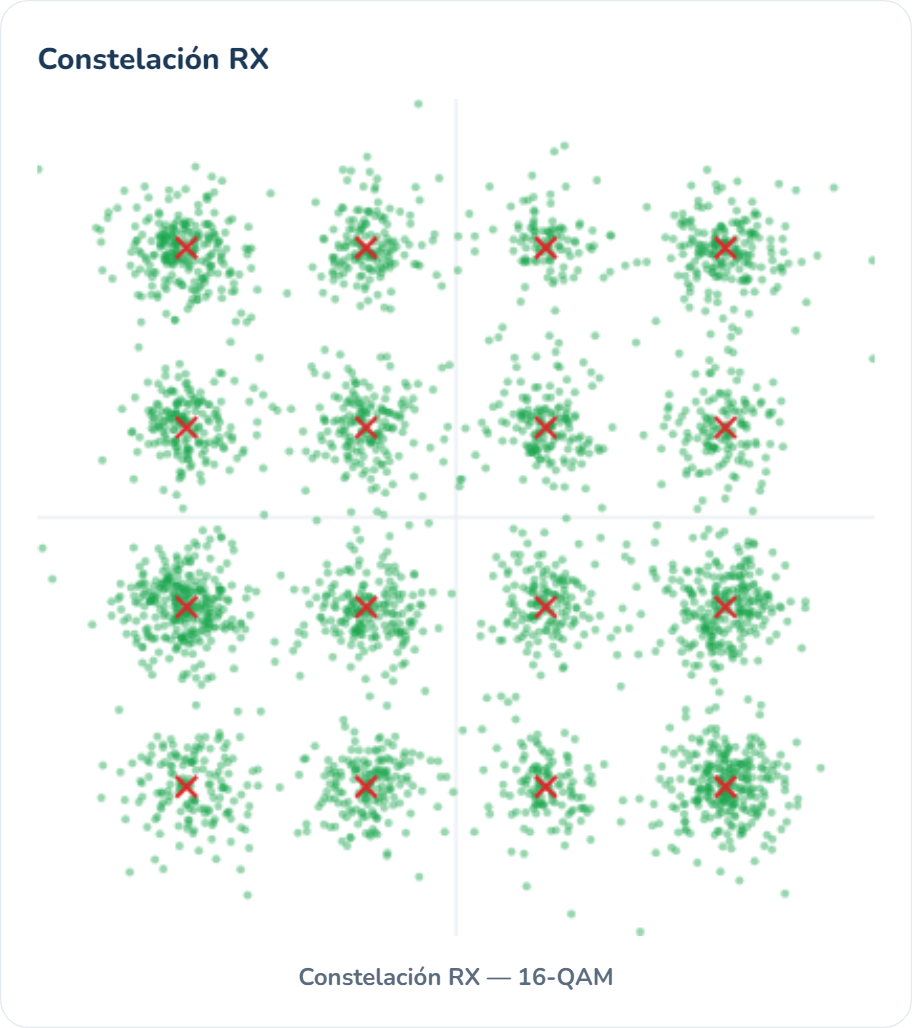
\includegraphics[width=0.65\textwidth]{img/constelacion.png}
\caption{Constelaci\'on de 16-QAM recibida tras la ecualizaci\'on Zero-Forcing (cruces rojas: s\'imbolos ideales; puntos verdes: s\'imbolos recibidos).}
\label{fig:const}
\end{figure}

\begin{figure}[H]
\centering
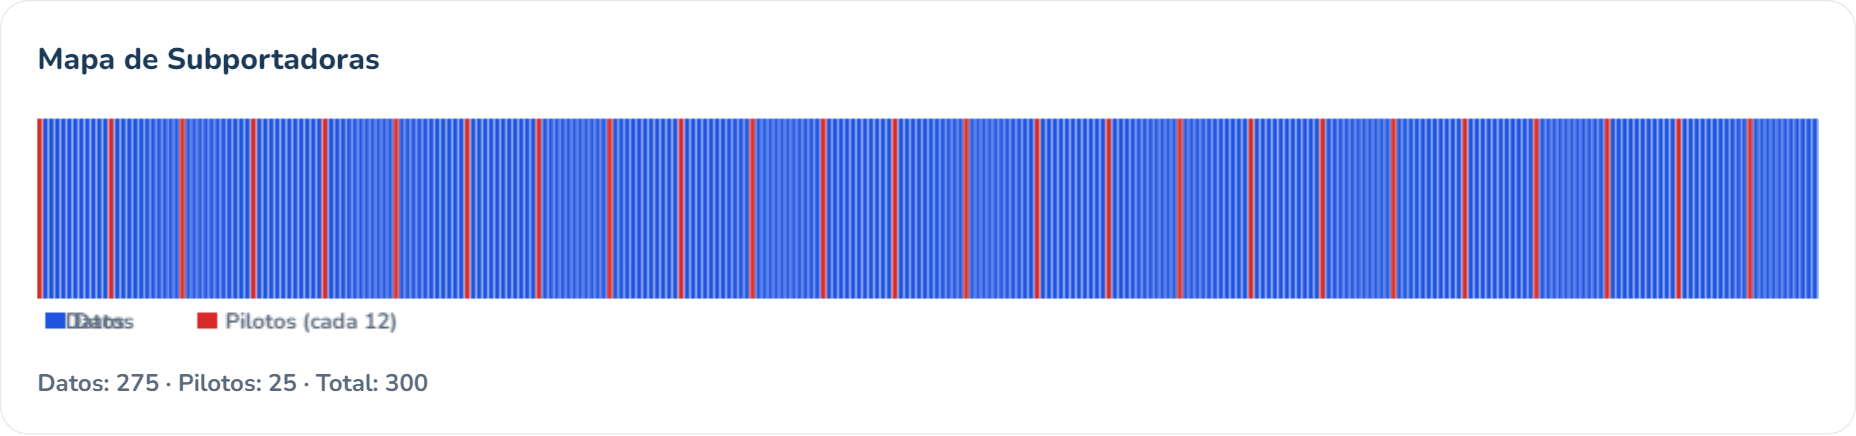
\includegraphics[width=0.95\textwidth]{img/mapa_subportadoras.png}
\caption{Mapa de las $300$ subportadoras: datos (azul) y pilotos (rojo, una de cada doce).}
\label{fig:mapasc}
\end{figure}

\subsection{Curvas BER frente a SNR (an\'alisis de Monte Carlo)}

La Fig.~\ref{fig:montecarlo} presenta las curvas de BER promedio frente a la SNR ($0$--$15$~dB) obtenidas con $10$ corridas independientes por punto y $50\,000$ bits aleatorios por corrida, con intervalos de confianza al $95\%$ calculados con la distribuci\'on $t$ de Student ($9$ grados de libertad). A diferencia de la Tabla~\ref{tab:sims}, aqu\'i las tres modulaciones se comparan a igualdad de SNR, por lo que se aprecia el orden te\'orico esperado: QPSK presenta la menor BER, seguida de 16-QAM y de 64-QAM, la m\'as sensible al ruido por tener la menor distancia m\'inima entre s\'imbolos. Todas las curvas decrecen mon\'otonamente con la SNR. Los intervalos de confianza son estrechos en la regi\'on de baja SNR y se ensanchan ligeramente a SNR altas, donde los errores escasean y la varianza relativa entre corridas aumenta.

\begin{figure}[H]
\centering
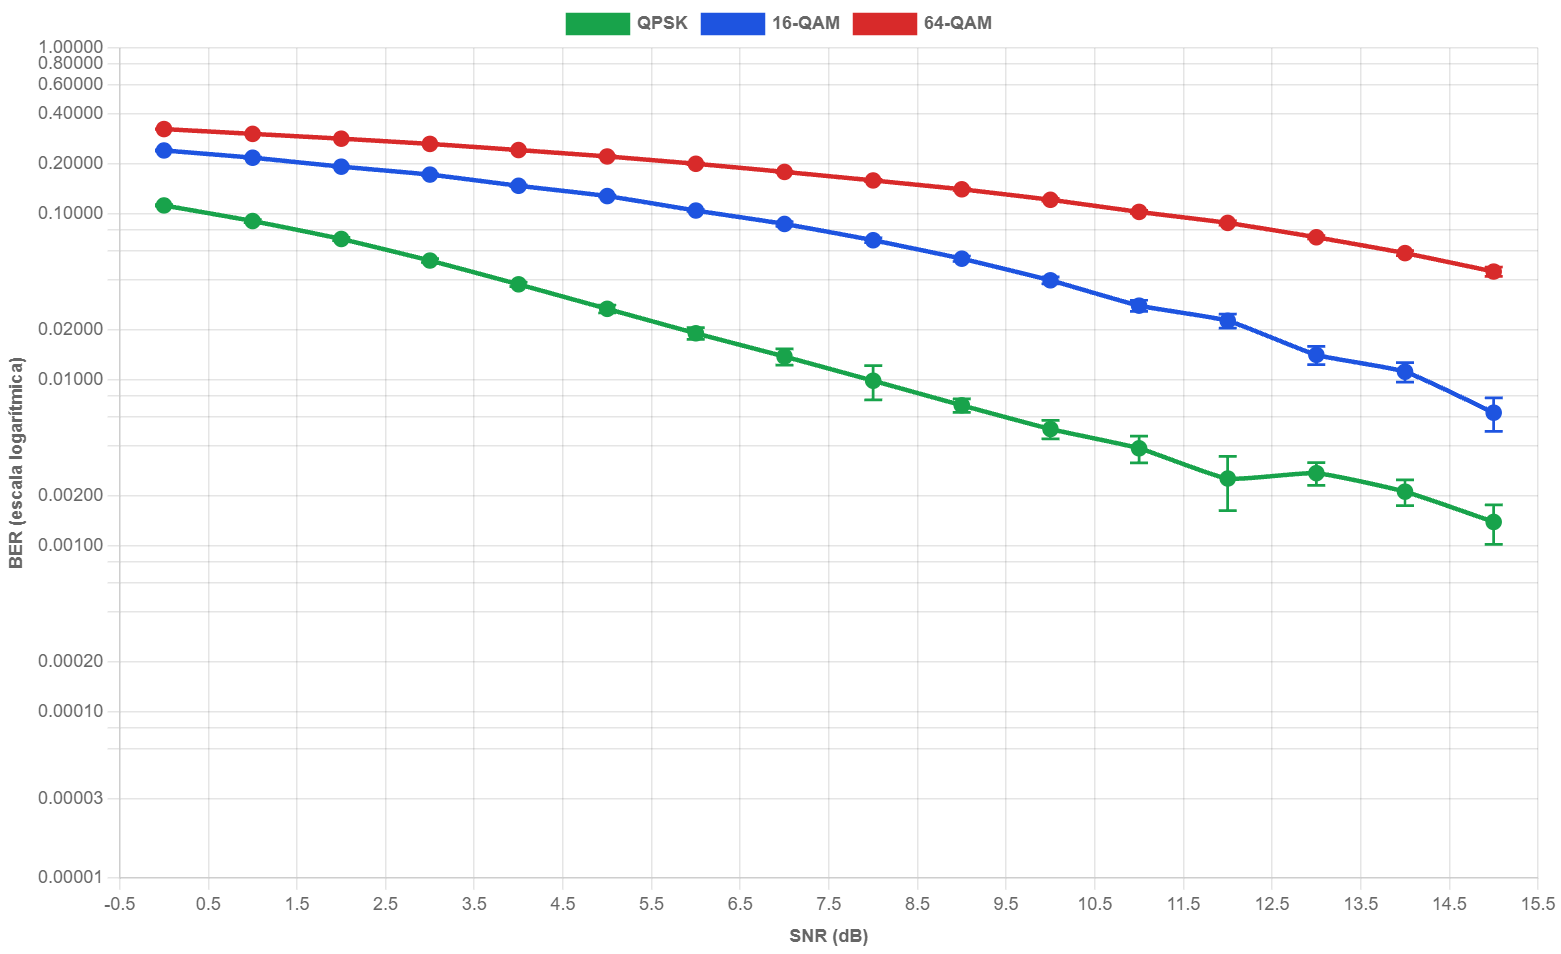
\includegraphics[width=0.9\textwidth]{img/montecarlo.png}
\caption{BER frente a SNR para QPSK, 16-QAM y 64-QAM (Monte Carlo, $10$ corridas por punto, IC al $95\%$ con $t$ de Student).}
\label{fig:montecarlo}
\end{figure}

\subsection{CCDF de la PAPR}

Finalmente, la Fig.~\ref{fig:papr} muestra la CCDF de la PAPR, es decir, la probabilidad de que la PAPR de un s\'imbolo OFDM supere un umbral dado, estimada sobre $1500$ s\'imbolos por modulaci\'on. Las tres curvas son pr\'acticamente coincidentes, lo que confirma que la PAPR de una se\~nal OFDM depende esencialmente del n\'umero de subportadoras y no del esquema de modulaci\'on de cada una. La probabilidad permanece cercana a la unidad hasta aproximadamente $7$~dB y luego decae con rapidez, alcanzando valores del orden de $10^{-3}$ en torno a $11$--$12$~dB. Estos picos elevados y poco frecuentes son los que obligan a dimensionar el amplificador de potencia con un margen (\textit{back-off}) adecuado para evitar distorsi\'on no lineal.

\begin{figure}[H]
\centering
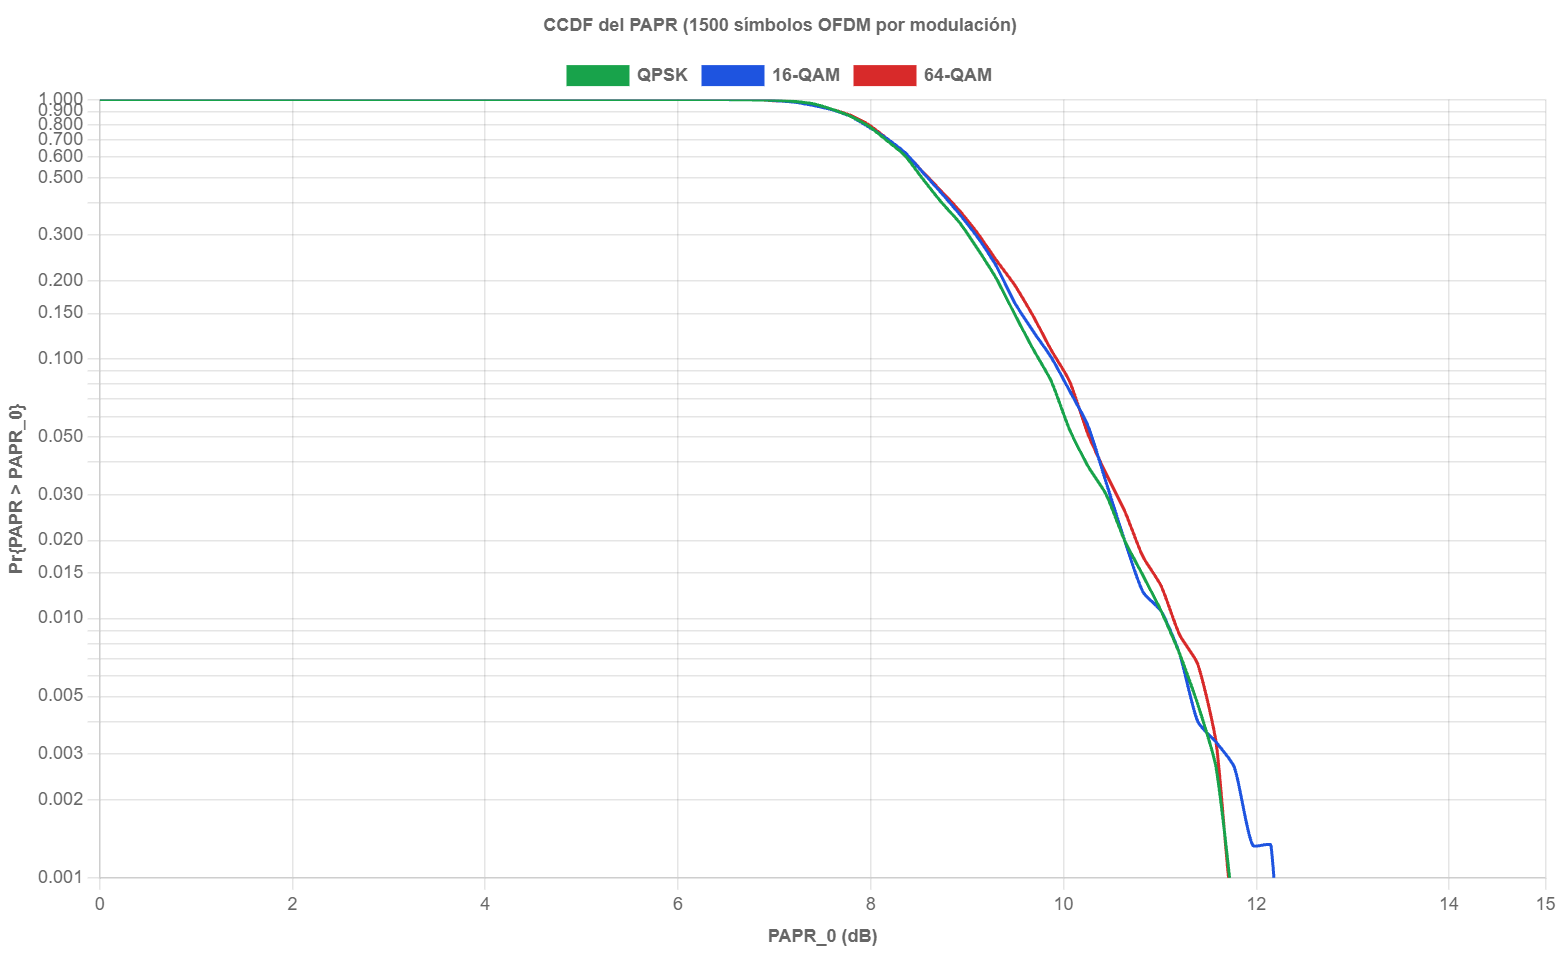
\includegraphics[width=0.9\textwidth]{img/papr.png}
\caption{CCDF de la PAPR para QPSK, 16-QAM y 64-QAM, estimada sobre $1500$ s\'imbolos OFDM por modulaci\'on.}
\label{fig:papr}
\end{figure}

\section{Conclusiones}

El simulador desarrollado reproduce de forma integral la cadena OFDM conforme a la numerolog\'ia de LTE, desde el mapeo de bits con codificaci\'on Gray hasta la recepci\'on con ecualizaci\'on Zero-Forcing sobre un canal Pedestrian~A con desvanecimiento de Rayleigh y ruido AWGN. Los resultados confirman que la ecualizaci\'on ZF es imprescindible para compensar la distorsi\'on multiplicativa del canal selectivo en frecuencia: gracias a ella, las constelaciones recibidas se reagrupan en torno a sus posiciones ideales y la imagen se recupera con una calidad que mejora al aumentar la SNR. Las transmisiones de imagen mostraron que 64-QAM con buena SNR ($30$~dB) recupera la imagen casi sin errores (BER ${\approx}9{,}8\times10^{-4}$), mientras que QPSK mantiene la imagen legible incluso en el borde de celda con SNR baja ($6$~dB), lo que ilustra el fundamento de la modulaci\'on adaptativa de LTE.

El an\'alisis de Monte Carlo, al comparar las tres modulaciones a igualdad de SNR, evidenci\'o el compromiso entre eficiencia espectral y robustez: la BER empeora al aumentar el orden de modulaci\'on (QPSK $<$ 16-QAM $<$ 64-QAM) debido a la reducci\'on de la distancia m\'inima entre s\'imbolos, y los intervalos de confianza al $95\%$ con la distribuci\'on $t$ de Student confirmaron la estabilidad estad\'istica de las estimaciones. Por \'ultimo, la CCDF de la PAPR result\'o pr\'acticamente independiente del esquema de modulaci\'on y dominada por el n\'umero de subportadoras, con valores de pico que superan los $11$~dB con probabilidad del orden de $10^{-3}$, lo que justifica la necesidad de un margen de operaci\'on (\textit{back-off}) en el amplificador de potencia.

\bibliographystyle{IEEEtran}
\bibliography{referencias}

\clearpage
\onecolumn
\newpage
\section*{Anexos}

\begin{figure}[H]
    \centering
    
\includegraphics[width=0.22\textwidth]{img/qr_sitio.png}
    \caption{C\'odigo QR del simulador OFDM desplegado: \texttt{https://ofdm.tesisucuenca.com}}
    \label{fig:qrsitio}
\end{figure}

\begin{figure}[H]
    \centering
    
\includegraphics[width=0.22\textwidth]{img/qr_repo.png}
    \caption{C\'odigo QR del repositorio del proyecto: \texttt{https://github.com/thyron001/ofdm}}
    \label{fig:qrrepo}
\end{figure}

\end{document}